\documentclass[a4paper,10pt]{article}
\usepackage[utf8]{inputenc}
\usepackage{tikz}

\usetikzlibrary{automata} %state machine stuff
\usetikzlibrary{positioning} %midway
\begin{document}

\begin{figure}
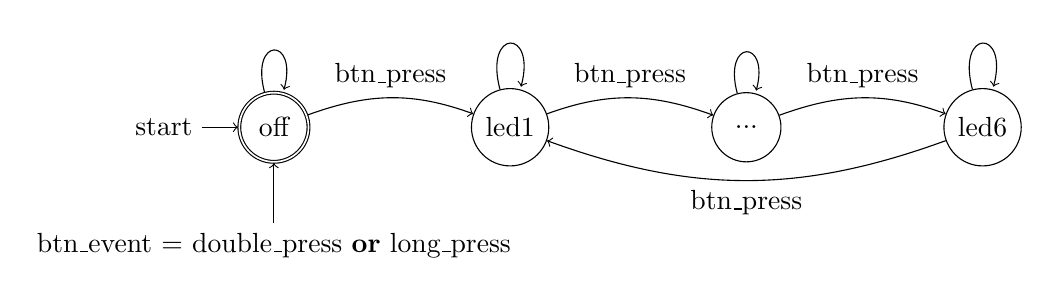
\begin{tikzpicture}[node distance=3cm]
 \node[initial,accepting,state,name=off ]    {off}; 
 \node[state,right of=off,     name=led1]    {led1};
 \node[state,right of=led1,    name=led_i]   {...};
 \node[state,right of=led_i,   name=led6]    {led6};
 
 
 \draw (off)   edge[loop above] (off)  ;
 \draw (led1)  edge[loop above] (led1) ;
 \draw (led_i) edge[loop above] (led_i);
 \draw (led6)  edge[loop above] (led6) ;
 
 \draw[->] (off)   to[out=20, in=160]   node[midway,above] {btn\_press}  (led1)   ;
 \draw[->] (led1)  to[out=20, in=160]   node[midway,above] {btn\_press}  (led_i)  ;
 \draw[->] (led_i) to[out=20, in=160]   node[midway,above] {btn\_press}  (led6)   ;
 \draw[->] (led6)  to[out=200,in=340]   node[midway,below] {btn\_press}  (led1)   ;
 
 \node[name = reset, below of=off,yshift=1.5cm] {btn\_event = double\_press \textbf{or} long\_press };
 \draw[->] (reset) to (off);
 
\end{tikzpicture}
\caption{Main state machine}
\end{figure}

\begin{figure}
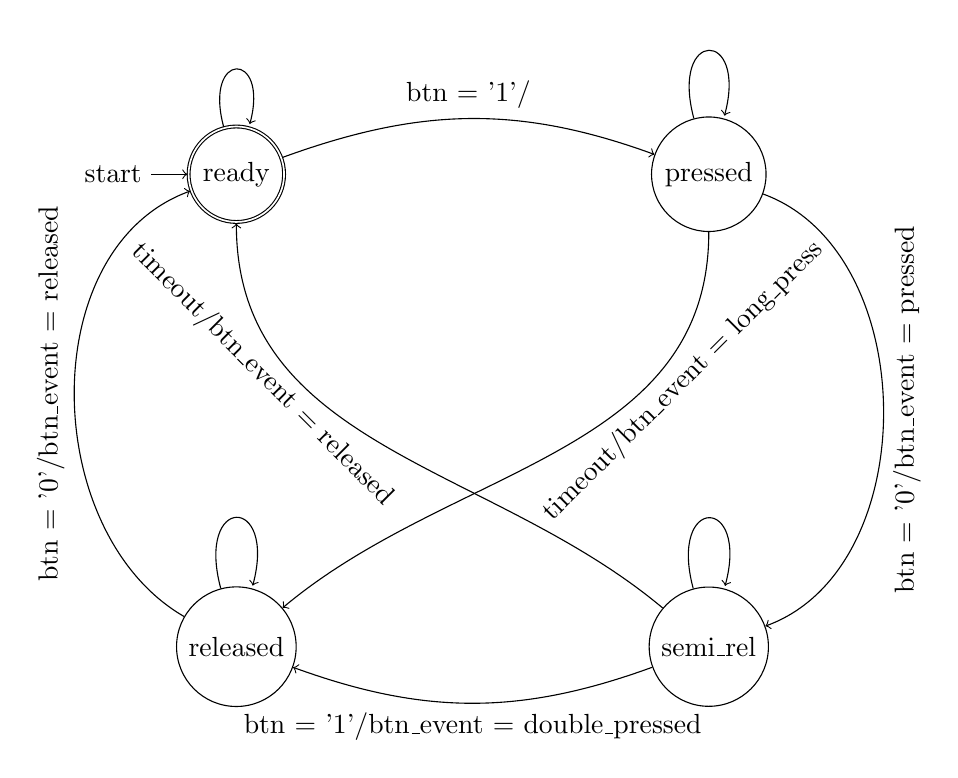
\begin{tikzpicture}[node distance=6cm]
 \node[initial,accepting,state,       name=ready ]         {ready}; 
 \node[state,right of=ready,          name=pressed]        {pressed};
 \node[state,below of=pressed,        name=semi-released]  {semi\_rel};
 \node[state,left of=semi-released,   name=released]       {released};
 
 \draw (ready)           edge[loop above] (ready)       ;
 \draw (pressed)         edge[loop above] (pressed)        ;
 \draw (semi-released)   edge[loop above] (semi-released)  ;
 \draw (released)        edge[loop above] (released) ;
 
 \draw[->] (ready)          to[out=20, in=160] node[midway,above]               {btn = '1'/}         (pressed)  ;
 \draw[->] (pressed)        to[out=340,in=20 ] node[midway,below,rotate=90]     {btn = '0'/btn\_event = pressed}          (semi-released) ;
 \draw[->] (pressed)        to[out=270,in=40 ] node[near start,below,rotate=45] {timeout/btn\_event = long\_press}        (released) ;
 \draw[->] (semi-released)  to[out=140,in=270] node[near end,below,rotate=-45]  {timeout/btn\_event = released}           (ready) ;
 \draw[->] (semi-released)  to[out=200,in=340] node[midway,below]               {btn = '1'/btn\_event = double\_pressed}  (released) ;
 \draw[->] (released)       to[out=150,in=200] node[midway,above,rotate=90]     {btn = '0'/btn\_event = released}         (ready) ;
\end{tikzpicture}
\caption{Button state machine}
\end{figure}

\begin{figure}
 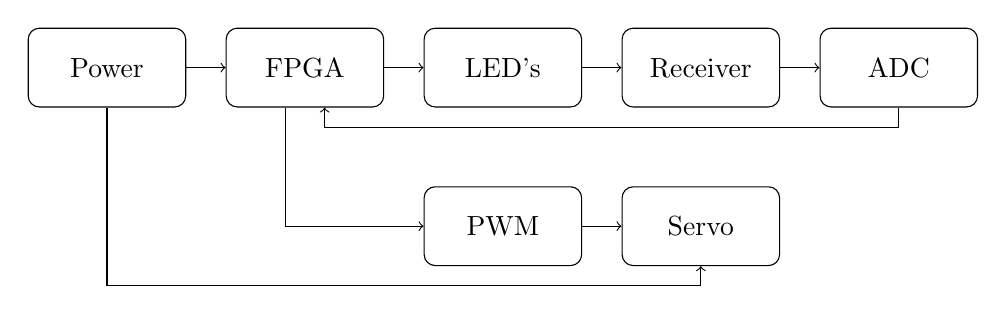
\begin{tikzpicture}
  \node[draw,rounded corners,minimum width=2cm,minimum height=1cm, name=power] {Power};
  \node[draw,rounded corners,minimum width=2cm,minimum height=1cm, name=fpga, right=0.5cm of power] {FPGA};
  \node[draw,rounded corners,minimum width=2cm,minimum height=1cm, name=led, right=0.5cm of fpga] {LED's};
  \node[draw,rounded corners,minimum width=2cm,minimum height=1cm, name=receiver, right=0.5cm of led] {Receiver};
  \node[draw,rounded corners,minimum width=2cm,minimum height=1cm, name=adc, right=0.5cm of receiver] {ADC};                                              
  \node[draw,rounded corners,minimum width=2cm,minimum height=1cm, name=pwm, below right=1cm and 0.5cm of fpga] {PWM};
  \node[draw,rounded corners,minimum width=2cm,minimum height=1cm, name=servo, right=0.5cm of pwm] {Servo};
  
  
  \draw[->] (power)    -- (fpga);
  \draw[->] (fpga)     -- (led);
  \draw[->] (led)      -- (receiver);
  \draw[->] (receiver) -- (adc);
  \draw[<-] (fpga.south) ++(0.25,0) -- ++(0,-0.25) -| (adc);
  
  \draw[->] (fpga.south) ++(-0.25,0) |- (pwm); %here
  \draw[->] (pwm) -- (servo);
  \draw[<-] (servo.south) -- ++(0,-0.25) -| (power);
  
 \end{tikzpicture}
\end{figure}


\end{document}
